\documentclass[12pt,a4paper]{article}
\usepackage{amsmath} % For advanced math formatting
\usepackage{tikz} % For drawing diagrams
\usepackage{geometry} % For adjusting page margins
\geometry{margin=1in}
\usetikzlibrary{shapes.geometric, arrows.meta, positioning}
\usepackage{enumitem} % For customising lists
\usepackage{siunitx} % For units

\pagenumbering{gobble} 

\title{ImprovementActivitySheetsCore}
\author{matthew.holmes111 }
\date{November 2025}

\begin{document}

\section*{Simplifying Ratios}
\emph{Simplify these ratios to their simplest form.}

\begin{enumerate}
\item \( 14 : 21 \)

\vspace{0.8cm}

\item \( 24 : 18 : 42 \)

\vspace{0.8cm}

\item \( 1.5 : 4.5 \)

\vspace{0.8cm}

\item \( \frac{2}{3} : \frac{4}{5} \)

\vspace{0.8cm}

\item A recipe for paint mix requires 600 ml of white paint, 250 ml of blue paint, and 150 ml of yellow paint. What is the ratio of white : blue : yellow paint in its simplest form?

\vspace{1.2cm}
\end{enumerate}

\vspace{3cm}

\section*{Sharing into Ratios}

Divide the quantities as described.

\begin{enumerate}
    \item Share 24 sweets between two children in the ratio 3:1.

    \item An amount of £80 is divided between two people in the ratio 3:2. How much does each person receive?

    \item 180 students are divided into three groups in the ratio 2:3:4. How many students are in each group?

    \item A piece of wood 2.4 meters long is cut into three pieces in the ratio 1:2:5. Find the length of each piece.

    \item A bag contains red, blue, and green marbles in the ratio 2:5:3. If there are 150 marbles in total, how many of each color are there?
\end{enumerate}

\newpage{}

\section*{Recipe Questions}

\begin{enumerate}
\item A recipe for 4 servings requires:
    \begin{itemize}
    \item 400g minced beef
    \item 2 onions (300g)
    \item 400g chopped tomatoes
    \item 150ml stock
    \end{itemize}
    How much of each ingredient is needed to make 10 servings?

\item A cookie recipe makes 15 cookies:
    \begin{itemize}
    \item 225g flour
    \item 150g butter
    \item 100g sugar
    \item 1 egg (50g)
    \end{itemize}
    How much of each ingredient is needed to make 35 cookies?

\item A salad dressing recipe for 2 portions:
    \begin{itemize}
    \item 60ml olive oil
    \item 30ml vinegar
    \item 10g mustard
    \item 5g honey
    \end{itemize}
    You need to make dressing for 7 portions. Calculate the new quantities.

\item The ingredients for a lemonade are in the ratio of \newline lemon juice : sugar : water = 2 : 1 : 8. To make 3.3 litres of lemonade, what volume of each ingredient is needed?

\item A curry recipe for 4 people calls for:
    \begin{itemize}
    \item 400g chicken
    \item 200g rice
    \item 300ml coconut milk
    \item 6 spices (individual items)
    \end{itemize}
    \begin{enumerate}
    \item Calculate the ingredient quantities needed to serve 11 people.
    \item You discover you only have 600g of chicken. What is the maximum number of people you can fully serve?
    \item Using the chicken from part (b), calculate the quantities for all other ingredients.
    \end{enumerate}
\end{enumerate}

\newpage{}

\section*{Direct Proportion}

\begin{enumerate}
    \item If 4 pencils cost 96p, find the cost of 7 pencils.

    \item A car travels 180 km in 3 hours. Assuming a constant speed, how far will it travel in 7 hours?

    \item The amount of paint needed is directly proportional to the area painted. If 2 litres of paint can cover 15 m$^2$, how many litres are needed to cover 90 m$^2$?

    \item The cost of a piece of rope is directly proportional to its length. A 2.5 metre piece of rope costs £1.35. Bob buys a piece of this rope and the cost is £3.24. What is the length of the rope he bought?

    \item The mass of a uniform metal bar is directly proportional to its length. A 1.2 m long bar has a mass of 4.5 kg. What is the mass of a similar bar that is 80 cm long?
\end{enumerate}

\vspace{6cm}


\section*{Best Buys}

\begin{enumerate}
\item Which is cheaper per gram: 200g of coffee for £5.40 or 350g for £8.75?

\item Pencils cost £4.80 for a pack of 12 or £11.00 for a pack of 30. Which pack offers better value per pencil?

\item Milk costs £2.85 for 2 liters or £6.50 for 5 liters. Which is the better buy?

\item A restaurant needs to buy rice. Option A: 8kg for £24.80. Option B: 15kg for £44.25. Option C: 25kg for £72.50. Which offers the best value per kilogram?

\item A car rental company charges: \\
Company X: £45 per day with unlimited mileage \\
Company Y: £35 per day plus £0.15 per mile \\
If you plan to drive 250 miles over 3 days, which company offers the better deal?
\end{enumerate}

\newpage{}

\section*{Scaling}

\begin{enumerate}

\item A scale drawing uses a ratio of 1:100. If a wall is drawn as 3.5 cm long, how long is the actual wall?

\item On a map with scale 1:50,000, two towns are 8.4 cm apart. What is the actual distance between them in kilometres?

\item 

If the rectangle below represents a garden drawn to scale 1:20, and it measures 4 cm by 3 cm in the drawing, what are the actual dimensions of the garden?
\begin{center}
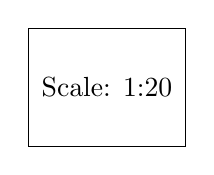
\begin{tikzpicture}[scale=0.5]
\draw (0,0) rectangle (4,3);
\node at (2,1.5) {Scale: 1:20};
\end{tikzpicture}
\end{center}

\item James is making a scale model of a car. The actual car is 4.2 meters long, and his model is 28 cm long. What scale is he using? Express your answer as a ratio in simplest form.

\item A map has a scale where 4 cm represents 5 km. Two cities appear 15.2 cm apart on the map. 
\begin{enumerate}
    \item What is the actual distance between the cities?
    \item What is the map scale expressed as a ratio?
    \item If another map uses scale 1:125,000, which map shows more detail (larger scale)?
\end{enumerate}

\item  The floor plan of a small room is 6 meters long and 4.5 meters wide. Using the squared background below, create a scale drawing of this room. Use a scale of \newline 1 cm : 1 m. Clearly label the dimensions on your drawing.
\begin{center}
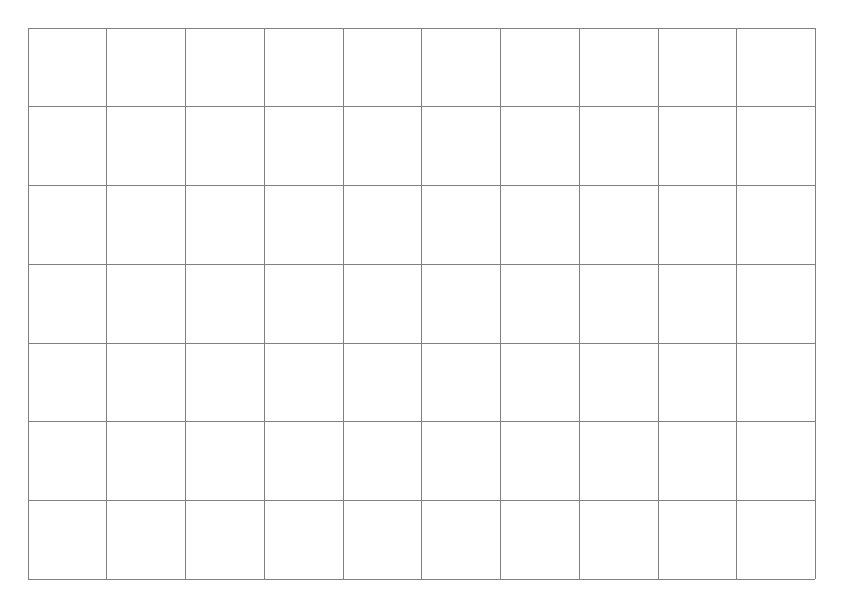
\begin{tikzpicture}
\draw[step=1cm, gray, very thin] (0,0) grid (10,7);
\end{tikzpicture}
\end{center}

\end{enumerate}

\newpage{}

\section*{Rates of Change}

\begin{enumerate}
    \item A cyclist travels \SI{45}{\kilo\metre} in 1 hour and 30 minutes. Calculate her average speed in \si{\kilo\metre\per\hour}.

    \item Water flows from a tap at a constant rate. It takes 3 minutes to fill a \SI{12}{\litre} watering can. At this rate, how long would it take to fill a \SI{90}{\litre} water butt?

    \item A train leaves London at 10:15 and arrives in York, \SI{320}{\kilo\metre} away, at 14:45. It stops for 10 minutes at a station halfway through the journey. Calculate the train's average speed for the whole journey, \textbf{including} the stop. What about the average speed when the train was in motion?

    \item A chemical reaction happens in a beaker. At the start, the beaker contains \SI{400}{\gram} of chemical A. The reaction uses up A at a rate of 4 grams per minute, how much chemical A is left in the beaker after 4 minutes?

    \item Sarah is driving on a motorway. She drives for \SI{30}{\minute} at an average speed of \SI{60}{\text{miles}\per\hour}. She then stops at a service station for 15 minutes. She completes her journey by driving for another \SI{45}{\minute} at an average speed of \SI{50}{\text{miles}\per\hour}.
    \begin{enumerate}
        \item Calculate the total distance of her journey.
        \item Calculate her average speed for the \textbf{whole journey}, including the stop.
    \end{enumerate}

\end{enumerate}

\vspace{3cm}

\section*{Problem Solving With Ratios}
\begin{enumerate}

    \item The ratio of red to blue marbles in a bag is $3:5$. If 8 red marbles are added, the ratio becomes $5:7$. How many blue marbles are there?

    \item The ratio of apples, bananas, and oranges in a fruit basket is $2:5:3$. After 4 apples and 2 bananas are added, the new ratio of apples to bananas to oranges is $4:6:3$ How many oranges are in the basket?

    \item The ratio of sugar to flour in a recipe is $2:9$. The ratio of flour to butter is $3:1$. Find the ratio of sugar to flour to butter.

    \item A sum of money is divided between Alex, Ben, and Chloe in the ratio $3:4:5$. If Ben receives £40 more than Alex, find the total sum of money.

    \item The points $A$, $B$, and $C$ lie on a straight line. The ratio of $AB$ to $BC$ is $3:2$. If $AB = 12$ cm, find the length of $AC$.

    \item A bag contains counters in three colours: red, yellow, and blue. The ratio of red to yellow is $3:4$. The ratio of yellow to blue is $5:6$. What fraction of the counters are blue?

\end{enumerate}

\end{document}
